\section{Chiral Anomalies}
%
Now we have a chiral gauge theory, SU(2)$_L\otimes$U(1)$_Y$, we can calculate loops! Renormalisation is just as in QCD: in particular the coupling runs (albeit very slowly); $\alpha(0) \approx 1/137$ but $\alpha(m_Z) \approx 1/128$ (determined from precision electroweak measurements at LEP). But when calculating loops we run into problems...
%
\subsection{Triangles (Adler-Bell-Jackiw, 1969)}
%
In QED, all diagrams with an odd number of photons vanish, because $V_\mu \to -V_\mu$ under $C$, as QED is $C$-invariant. Using $V$ to denote a vector vertex $\gamma^\mu$ and $A$ to denote an axial vector vertex $\gamma^\mu \gamma^5$, this means that 
\newline
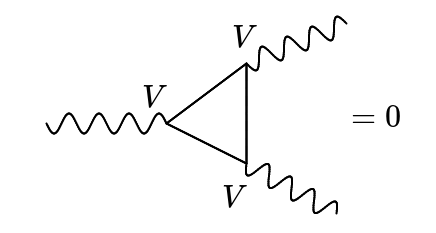
\includegraphics[width=0.4\linewidth]{figs/39a.png}
\newline
but for chiral theories, $C$ is not a symmetry so the triangle graphs are non-zero. The simplest example is the following.
\newline
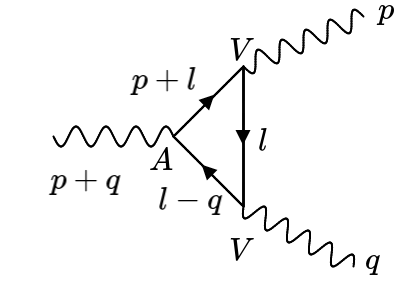
\includegraphics[width=0.4\linewidth]{figs/39b.png}
\newline
Note that this is the same as the crossed version of the graph, because loop momentum $l$ is integrated over. Breaking down the matrix element like
\begin{equation}
\mathcal{M} = \epsilon_\rho(p+q)\epsilon_\mu^*(p)\epsilon_\nu^*(q)\mathcal{M}^{\rho \mu \nu}(p,q),
\end{equation}
we can write
\begin{equation}
\begin{split}
\mathcal{M}^{\rho \mu \nu}(p,q) &= - (-ig)^3)i^3 \int \frac{d^4l}{(2\pi)^4}\ tr \frac{(\gamma^\rho \gamma^5)(\slashed{p} + \slashed{l})\gamma^\mu \slashed{l} \gamma^\nu (\slashed{l} - \slashed{q})}{(p+l)^2l^2(l-q)^2} \\
&= - g^3 \int \frac{d^4l}{(2\pi)^4}\ tr \frac{N^{\rho \mu \nu}}{(p+l)^2l^2(l-q)^2}, 
\end{split}
\end{equation}
where the fermion loop contributes an additional $-$ sign. Note that using $(\gamma^5)^2=1$,
\begin{equation}
N^{\rho \mu \nu} = tr\bigg((\gamma^\rho \gamma^5)(\slashed{p} + \slashed{l})\gamma^\mu \gamma^5 \slashed{l} \gamma^\nu \gamma^5 (\slashed{l} - \slashed{q})\bigg),
\end{equation}
so $AAA=AVV$, but $AAV=VVV=0$, so evaluating $AVV$ is sufficient to cover all cases. 

Considering the relevant Ward identities, conservation of vector current implies $p_\mu \mathcal{M}^{\rho \mu \nu}=0$, $q_\nu \mathcal{M}^{\rho \mu \nu}=0$; and conservation of axial vector current implies $(p+q)_\rho \mathcal{M}^{\rho \mu \nu} = 0$. Let's consider the axial current first:
\begin{equation}
\begin{split}
(p+q)_\rho N^{\rho \mu \nu} &=  tr(\slashed{l}-\slashed{q})(\slashed{p} + \slashed{q})\gamma^5(\slashed{p}+\slashed{l})\gamma^\mu \slashed{l} \gamma^\nu \\
&= tr \gamma^5(\slashed{l}-\slashed{q})(\slashed{p}+\slashed{l}-(\slashed{l}-\slashed{q}))(\slashed{p}+\slashed{l})\gamma^\mu \slashed{l} \gamma^\nu \\
&= tr \gamma^5((\slashed{l}-\slashed{q})(p+l)^2-(\slashed{p}+\slashed{l})(l-q)^2)\gamma^\mu \slashed{l} \gamma^\nu \\
&= 4i\epsilon^{\alpha \mu \beta \nu}((p+l)^2(l-q)_\alpha l_\beta - (l-q)^2(p+l)_\alpha l_\beta) \\
&= +4i\epsilon^{\mu \nu \alpha \beta}((p+l)^2 q_\alpha l_\beta + (l-q)^2 p_\alpha l_\beta),
\end{split}
\end{equation}
